
\section{An improved Metropolis-Hasting algorithm}
%\vspace{-.05in}
Our main idea is to symmetrize the probability of $W$ under the old and proposed parameters, so that $P(W|\theta)$ disappears from the acceptance ratio. 
Now, the probability of accepting a proposal $\vartheta$ depends only on the prior probabilities of $\theta$ and $\vartheta$, as well as how well they both explain the data.
This is in contrast to the previous algorithm, where one must also factor in how well each explains the current value of the grid $W$.
This results in a significantly more efficient, and also a simpler MCMC scheme.
%This forms the main contribution of this paper.

\begin{algorithm} %[H]
   \caption{Symmetrized MH for parameter inference for MJPs }
   \label{alg:MH_improved}
  \begin{tabular}{l l}
   \textbf{Input:  } & \text{The observations $X$,}
                      \text{the MJP path $S(t) = (S, T)$, parameters $\theta$} and $\pi_0$.\\ 
                     & \text{A  Metropolis-Hasting proposal $q(\cdot | \theta)$}.\\
   \textbf{Output:  }& \text{A new MJP trajectory $S'(t) = (S', T')$, 
                            new MJP parameters $\theta'$}.\\
   \hline
   \end{tabular}
   \begin{algorithmic}[1]
      \State Sample $\vartheta \sim q(\cdot| \theta)$, and 
      set %$\Omega = \max_i A_i(\theta) + \max_i A_i(\theta^*)$. 
	$\Omega \assign \Omega(\theta) + \Omega(\vartheta)$ for some function 
    $\Omega(\theta) \ge \max_s A_s(\theta)$.
      %In the case of uniformization, we
      %have a single $\Omega$ for all states, with $\Omega = \max_i A_i(\theta) + \max_i A_i(\theta^*)$.
      %, with $h(\theta) > max_s{|A_s(\theta)|}$, $h(\theta^*) > max_s{|A_s(\theta^*)|}$ using some deterministic function $h$.
      \State { Simulate the thinned times $U$ } from a rate-$(\Omega-A_{S(t)})$ Poisson process : 
\begin{align*}
  U \sim \text{PoissProc}(\Omega - A_{S(t)}) 
\end{align*}
    \State Set $W = T \cup U$ and discard MJP states.
    \State The current MCMC state-space is $(W,\theta,\vartheta)$. 
    Propose swapping $\theta$ and $\vartheta$, so the new state-space is $(W,\vartheta,\theta)$. 
     Accept this with probability 
     $
     \text{acc} 
        =  1 \wedge \frac{P(X| W,\vartheta,\theta)P(\vartheta)q(\theta|\vartheta)}
        {P(X| W,\theta, \vartheta)P(\theta) q(\vartheta|\theta)}.
        $
        \State \textbf{Forward pass:} Set $B(\theta,\vartheta) = I + \frac{A(\theta)}{\Omega(\theta, \vartheta)}$ and $\fwd^{\theta, \vartheta}_0(\cdot) = \pi_0$.
    %Sequentially update $\fwd^{\theta,\vartheta}_i(\cdot)$ at $w_i \in W$ as: 
    $$\textbf{for } i=1\rightarrow |W|\textbf{ do:} \quad \fwd^{\theta,\vartheta}_i(s') = \sum_{s \in \cS} \ell_{i-1}(s) \cdot \fwd^{\theta,\vartheta}_{i-1}(s)\cdot B_{ss'}(\theta,\vartheta), \quad \forall s' \in \cS.\qquad\qquad\quad $$
    Similarly, for $B(\vartheta,\theta) = I + \frac{A(\vartheta)}{\Omega(\vartheta, \theta)}$, calculate $\fwd^{\vartheta,\theta}_i(\cdot)$ for all $w_i \in W$.
    \State The current MCMC state-space is $(W,\theta,\vartheta)$. 
    Propose to swap $\theta$ and $\vartheta$, %so the new state-space is $(W,\vartheta,\theta)$. 
     and accept with probability 
     $
     \text{acc} 
        =  1 \wedge \frac{P(X| W,\vartheta,\theta)P(\vartheta)q(\theta|\vartheta)}
        {P(X| W,\theta, \vartheta)P(\theta) q(\vartheta|\theta)}.
        $
        Here, $P(X|W,\theta,\vartheta) = \sum_{s \in \cS} \fwd^{\theta,\vartheta}_{|W|}(s)$, and $P(X|W,\vartheta,\theta) = \sum_{s \in \cS} \fwd^{\vartheta,\theta}_{|W|}(s)$.
    Write the new MCMC state as $(W,\theta',\vartheta')$.
    \State \textbf{Backward pass:}
    Set $v_{|W|} \sim \bck^{\theta',\vartheta'}_{|W|}(\cdot)$, where $\bck^{\theta',\vartheta'}_{|W|}(s) \propto \fwd^{\theta',\vartheta'}_{|W|}(s)\cdot\ell_{|W|}(s) \quad \forall s \in \cS.$ 
    %For the new transition matrix $B(\theta',\vartheta')$,     
    $$\hspace{-.15in} \textbf{for } i=(|W|-1)\rightarrow 0\textbf{ do:} \ v_i \sim \bck^{\theta',\vartheta'}_i(\cdot), \text{where } 
    \bck^{\theta',\vartheta'}_i(s) \propto \fwd^{\theta',\vartheta'}_i(s)\cdot B_{sv_{i+1}}(\theta',\vartheta') \cdot \ell_i(s)  \ \forall s \in \cS.$$
    
%    Sample a path $\tilde{V}$, from a discret-time Markov chain with $|W| + 1$ steps, using FFBS algorithm. The transition matrix of the Markov chain is $B = (I + \frac{A(\tilde{\theta})}{\Omega})$ while the initial distribution over states is $\pi_0$. The likelihood of state $s$ at step $i$ is 
%    $$ L_i(s) = P(Y_{[w_i, w_{i + 1})} | S(t) = s \; for\; t \in [w_i, w_{i + 1})) = \prod_{j: t_j \in [w_i, w_{i + 1})}p(y_{t_j} | S(t_j) = s).$$\\
%%(i.e. $V(i) \sim P(V |  \theta(i), W(i - 1), y).$) Then delete all the virtual jumps to get $S(i), T(i) .$\\
    \State Let $T'$ be the set of times in $W$ when $V$ changes state. Define $S'$ as the corresponding set of state values. Return $(S', T', \theta')$.
\end{algorithmic}
\end{algorithm}


\setlength{\unitlength}{0.8cm}
  \begin{figure}[h!]
  \centering
  \begin{minipage}[!hp]{0.45\linewidth}
  \centering
    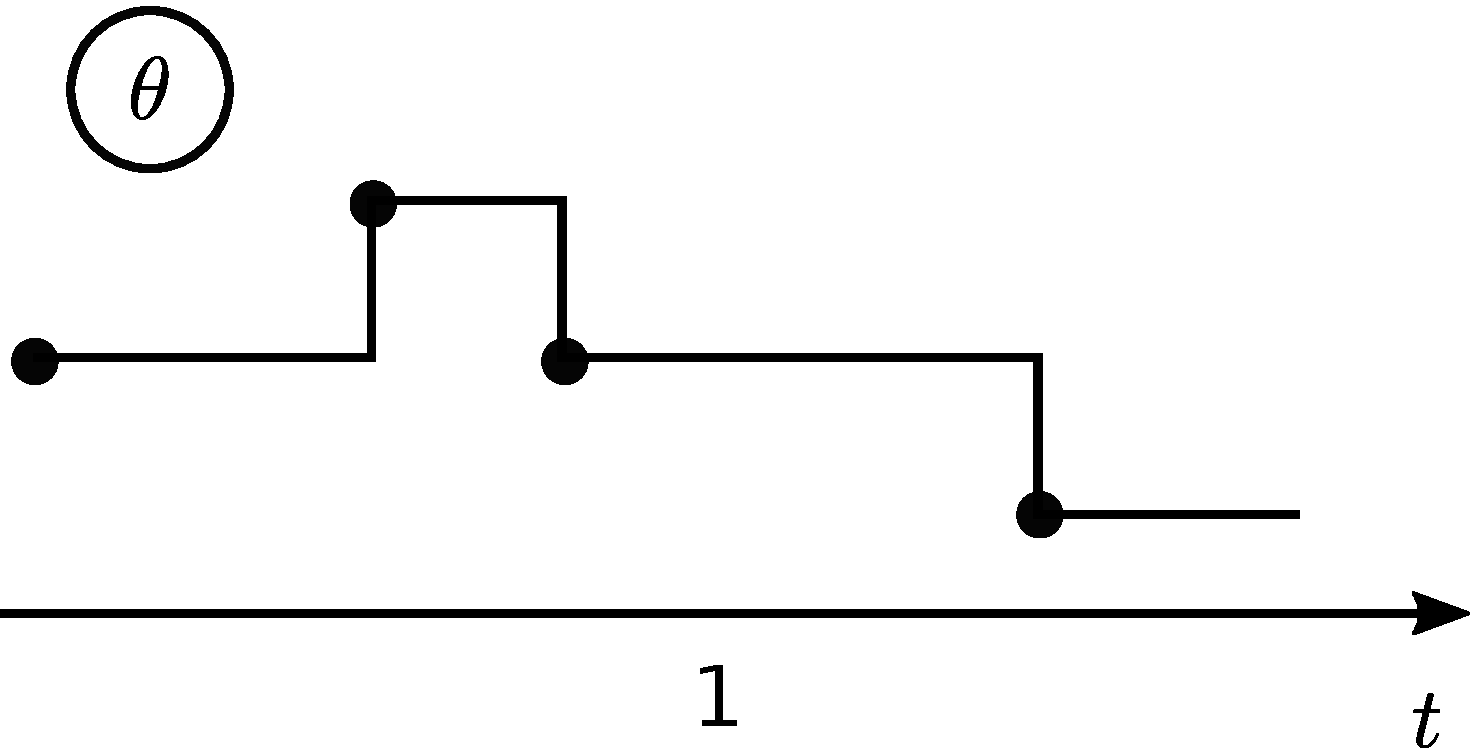
\includegraphics [width=0.90\textwidth, angle=0]{figs/plot0.pdf}
      \end{minipage}
  \begin{minipage}[hp]{0.45\linewidth}
  \centering
    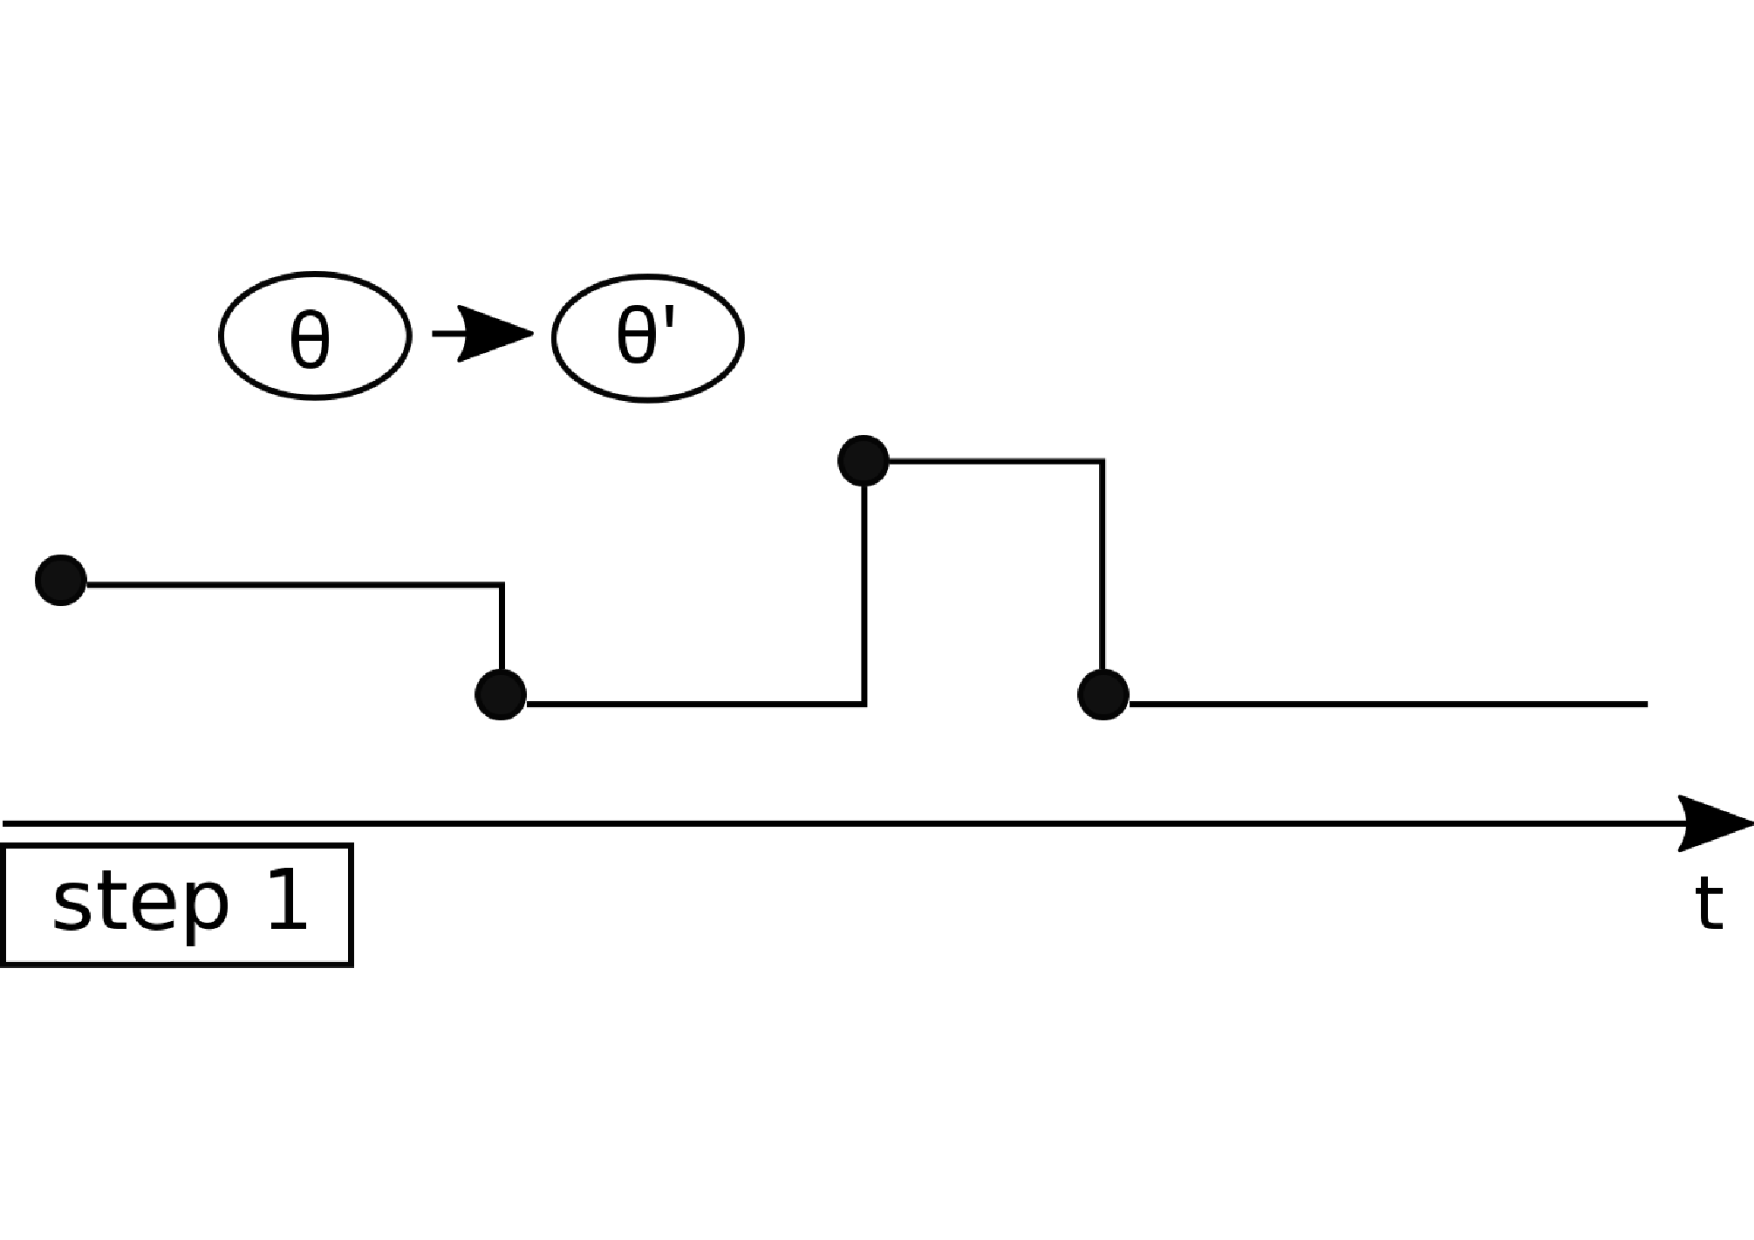
\includegraphics [width=0.90\textwidth, angle=0]{figs/plot1.pdf}
    \vspace{-0 in}
  \end{minipage}
  \begin{minipage}[hp]{0.45\linewidth}
  \centering
    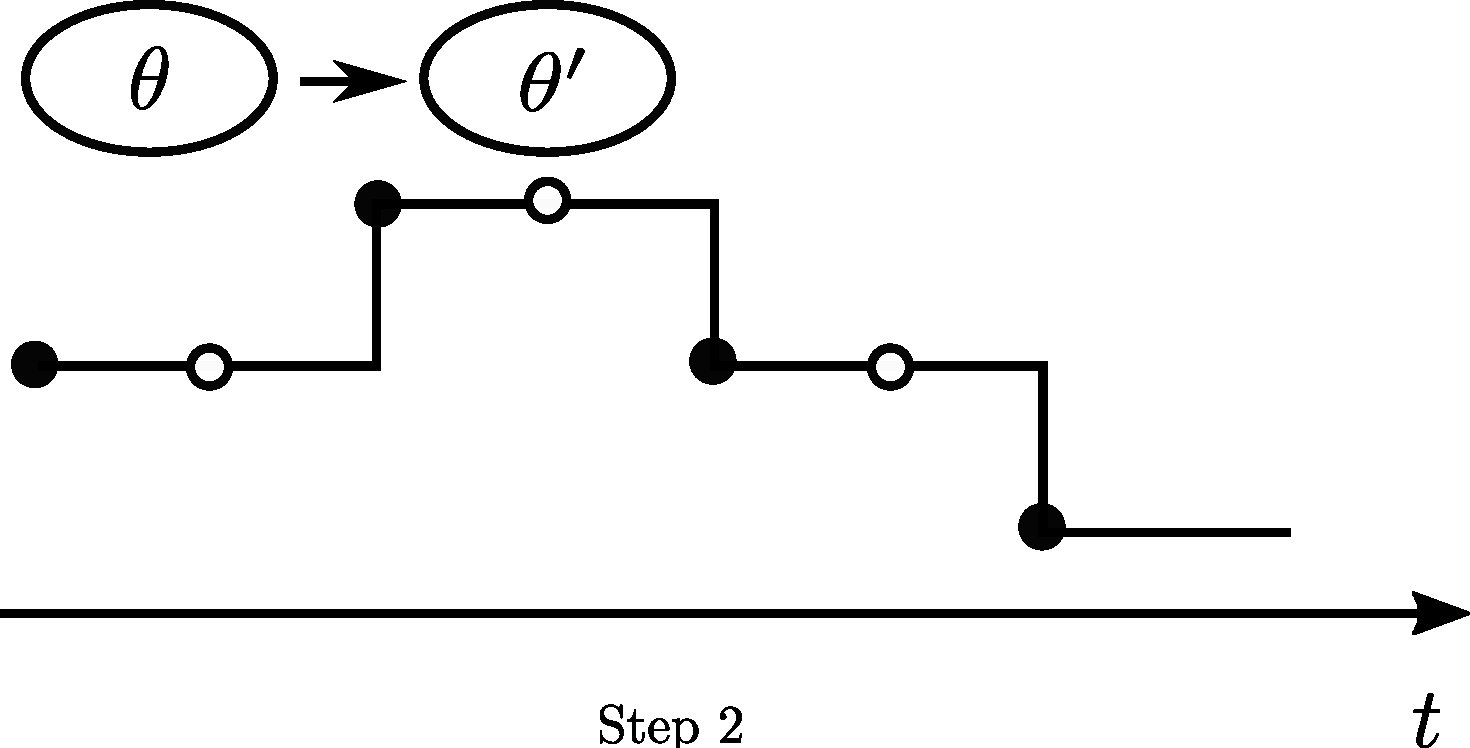
\includegraphics [width=0.90\textwidth, angle=0]{figs/plot2.pdf}
    \vspace{-0 in}
  \end{minipage}
  \begin{minipage}[hp]{0.45\linewidth}
  \centering
    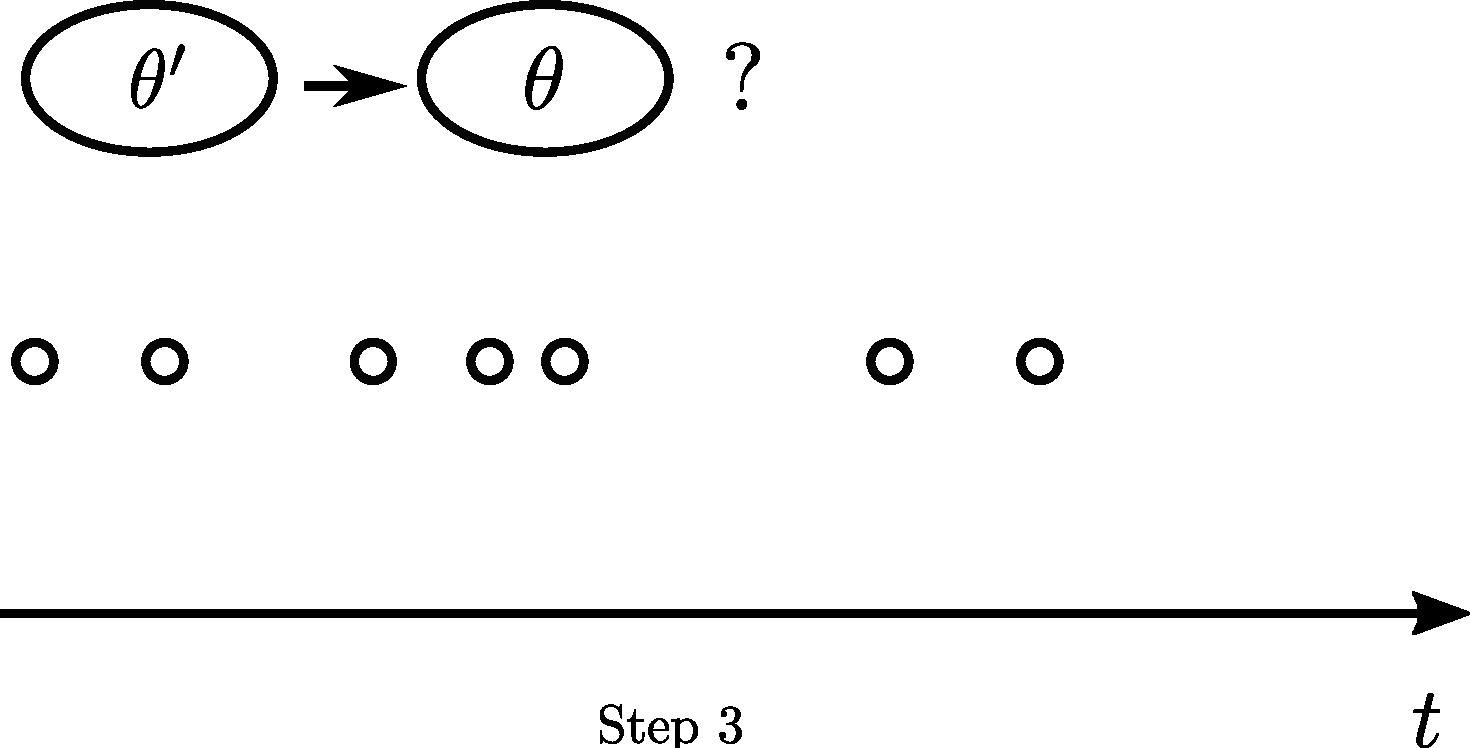
\includegraphics [width=0.90\textwidth, angle=0]{figs/plot3.pdf}
    \vspace{-0 in}
  \end{minipage}
% \begin{minipage}[hp]{0.45\linewidth}
% \centering
%   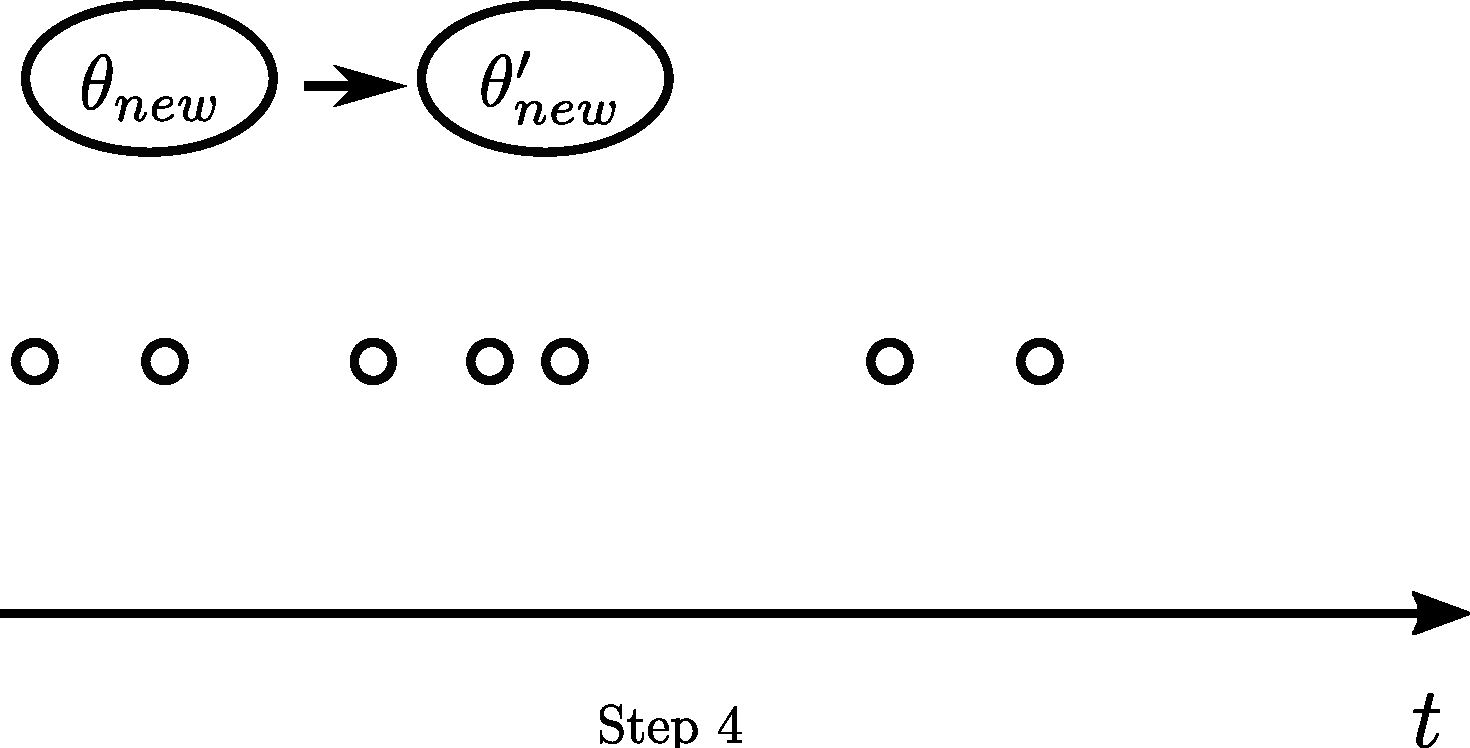
\includegraphics [width=0.70\textwidth, angle=0]{figs/plot4.pdf}
%   \vspace{-0 in}
% \end{minipage}
  \begin{minipage}[hp]{0.45\linewidth}
  \centering
    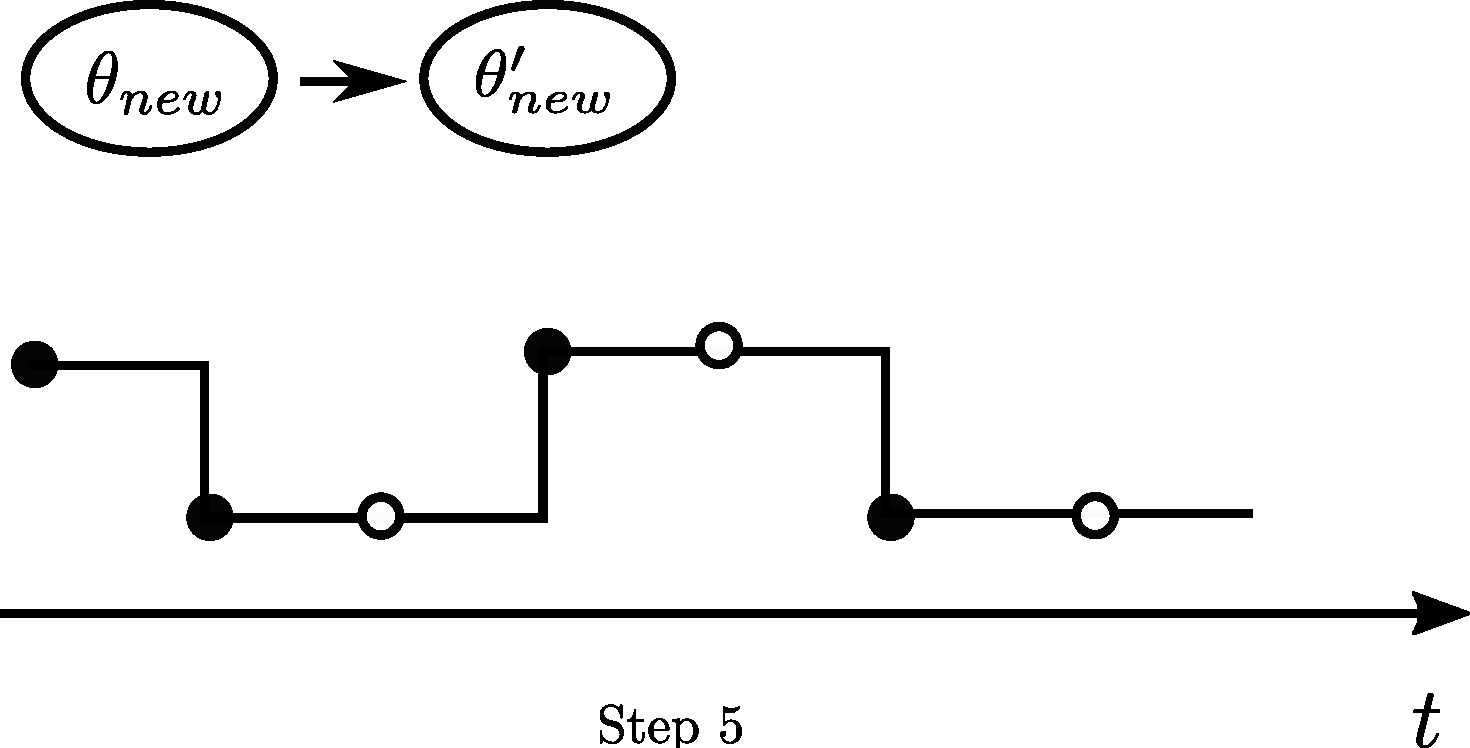
\includegraphics [width=0.90\textwidth, angle=0]{figs/plot5.pdf}
    \vspace{-0 in}
  \end{minipage}
  \begin{minipage}[hp]{0.45\linewidth}
  \centering
    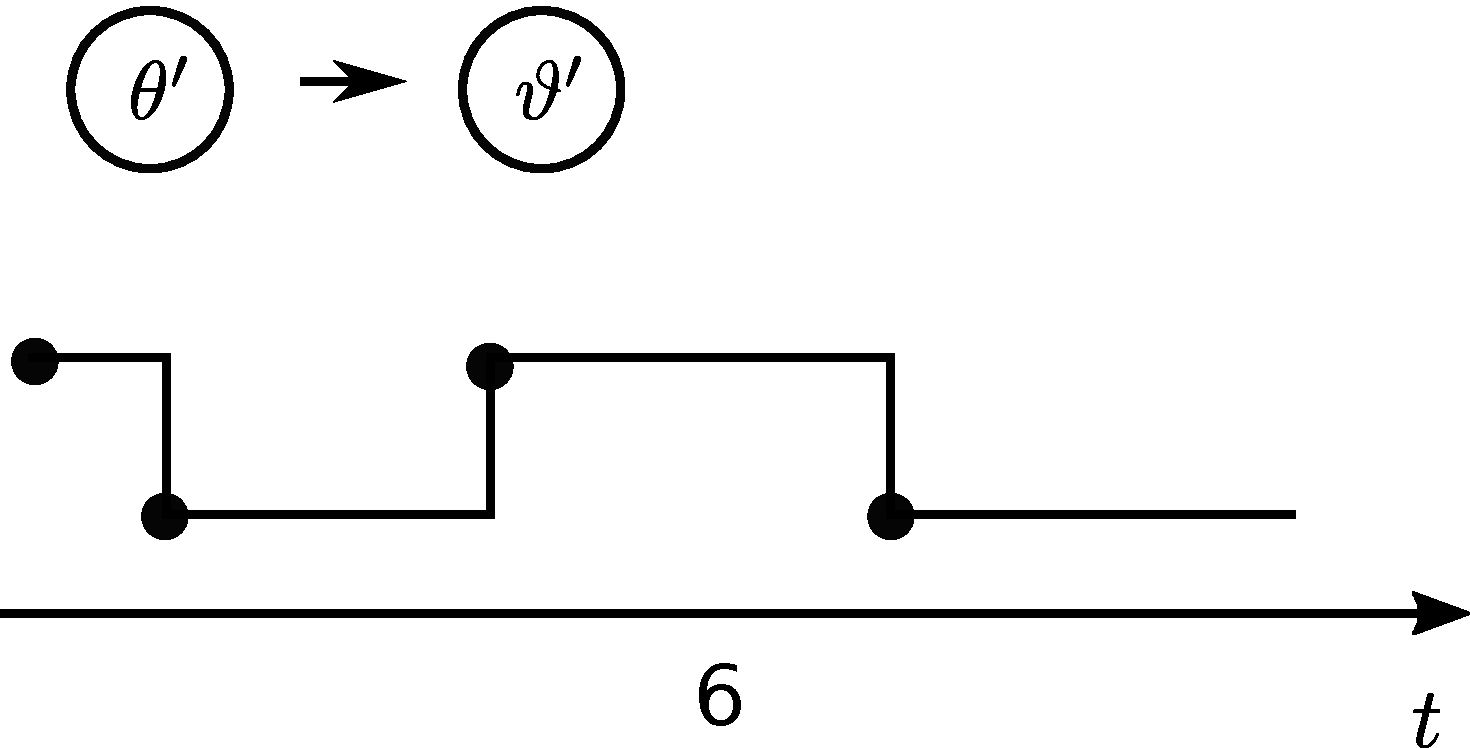
\includegraphics [width=0.90\textwidth, angle=0]{figs/plot6.pdf}
  \end{minipage}
    \caption{Proposed MH algorithm: Steps 0-3: Starting with a trajectory and parameter $\theta$,
      simulate an auxiliary parameter $\theta^*$, and then the thinned events
      $U$ from a rate $\Omega(\theta) + \Omega(\theta^*) - A_{S(t)}$ Poisson
      process. Step 4: Propose swapping $\theta$ and $\theta^*$. Step 5:
      Run a forward pass to accept or reject this proposal, and use the accepted
    parameter to simulate a new trajectory. Step 6: Discard the thinned events.} 
   \label{fig:MH_improved}
  \end{figure}
As before, the MCMC iteration begins with the pair $(S(t), \theta)$. 
Instead of simulating the Poisson events $U$, we first generate a new 
parameter $\vartheta$ from $q(\vartheta|\theta)$. Treat this as an 
auxiliary variable, so that the augmented space now is the triplet 
$(S(t), \theta,\vartheta)$. We pretend $S(t) \equiv (S,T)$ was sampled by  
uniformization, where the dominating Poisson rate $\Omega$ equals 
$(\Omega(\theta) + \Omega(\vartheta))$ instead of just $\Omega(\theta)$:
recall any choice greater than $\max_s A_s$ is valid.
Now the set of thinned events $U$ is piecewise-constant
Poisson with intensity $\Omega(\theta) + \Omega(\vartheta) - 
A_{S(t)}$. Following algorithm~\ref{alg:Unif_gibbs} or~\cite{RaoTeh13}, 
the {\em a priori} probability of the reconstructed set $W = U \cup T$, 
$P(W|\theta,\vartheta)$, is a homogeneous Poisson 
%the union of $U$ with the actual trajectory transition times $T$, 
process with rate $\Omega(\theta) + \Omega(\vartheta)$. Discard all 
MJP state information, so that the MCMC state space is $(W, \theta, \vartheta)$,
and propose swapping $\theta$ with $\vartheta$. 
Observe from
symmetry that the Poisson skeleton $W$ has the same probability both
before and after this proposal, so that unlike the previous scheme,
the ratio $P(W|\vartheta)/P(W|\theta)$ equals $1$.  This simplifies 
computation, and significantly improves mixing.
The acceptance probability 
%depends only on the probability of the observations
%under both set of parameters, %as we can use the forward-backward algorithm
%to calculate this. Our acceptance probability 
equals
$ 
  \min\left(1, \frac{P(X,\vartheta)q(\theta|\vartheta)}
   {P(X,\theta)q(\vartheta|\theta)}\right) = 
  \min\left(1, \frac{P(X|\vartheta)p(\vartheta)q(\theta|\vartheta)}
   {P(X|\theta)p(\theta)q(\vartheta|\theta)}\right).
   $
   The terms $P(X|\vartheta)$ and  $P(X|\theta)$ can be calculated by 
   running a forward pass of the forward-backward algorithm, and after
   accepting or rejecting the proposal, a new trajectory is sampled by
   completing the backward pass. Finally, the thinned events are
   discarded. See Algorithm~\ref{alg:MH_improved} and 
   figure~\ref{fig:MH_improved}. % for details. 

